\newpage
\subsection{Tidal harmonics to compliment aggregation with nontidal forecasts}
\label{S:plan_insitu_analysis}

\subsubsection{Problem and motivation}
Tidal harmonic predictions are often not treated as stand-alone forecast products. 
A recently developed scenario is the aggregation of harmonic tides with \BL{} sea level forecasts.\\

Following the discussion in the Literature Review [Section \ref{S:REVIEW}] there is reason to expect that aggregation may require measures to account for the `overlap' between heterogeneous forecast systems.   In fact, developmental aggregated forecasts (eg. Figure \ref{fig:aggregated_fc}) have been produced by modifying standard harmonic predictions.   It is now relevant to understand issues associated with such modifications in greater detail.\\



\begin{figure}[h]
\begin{center}
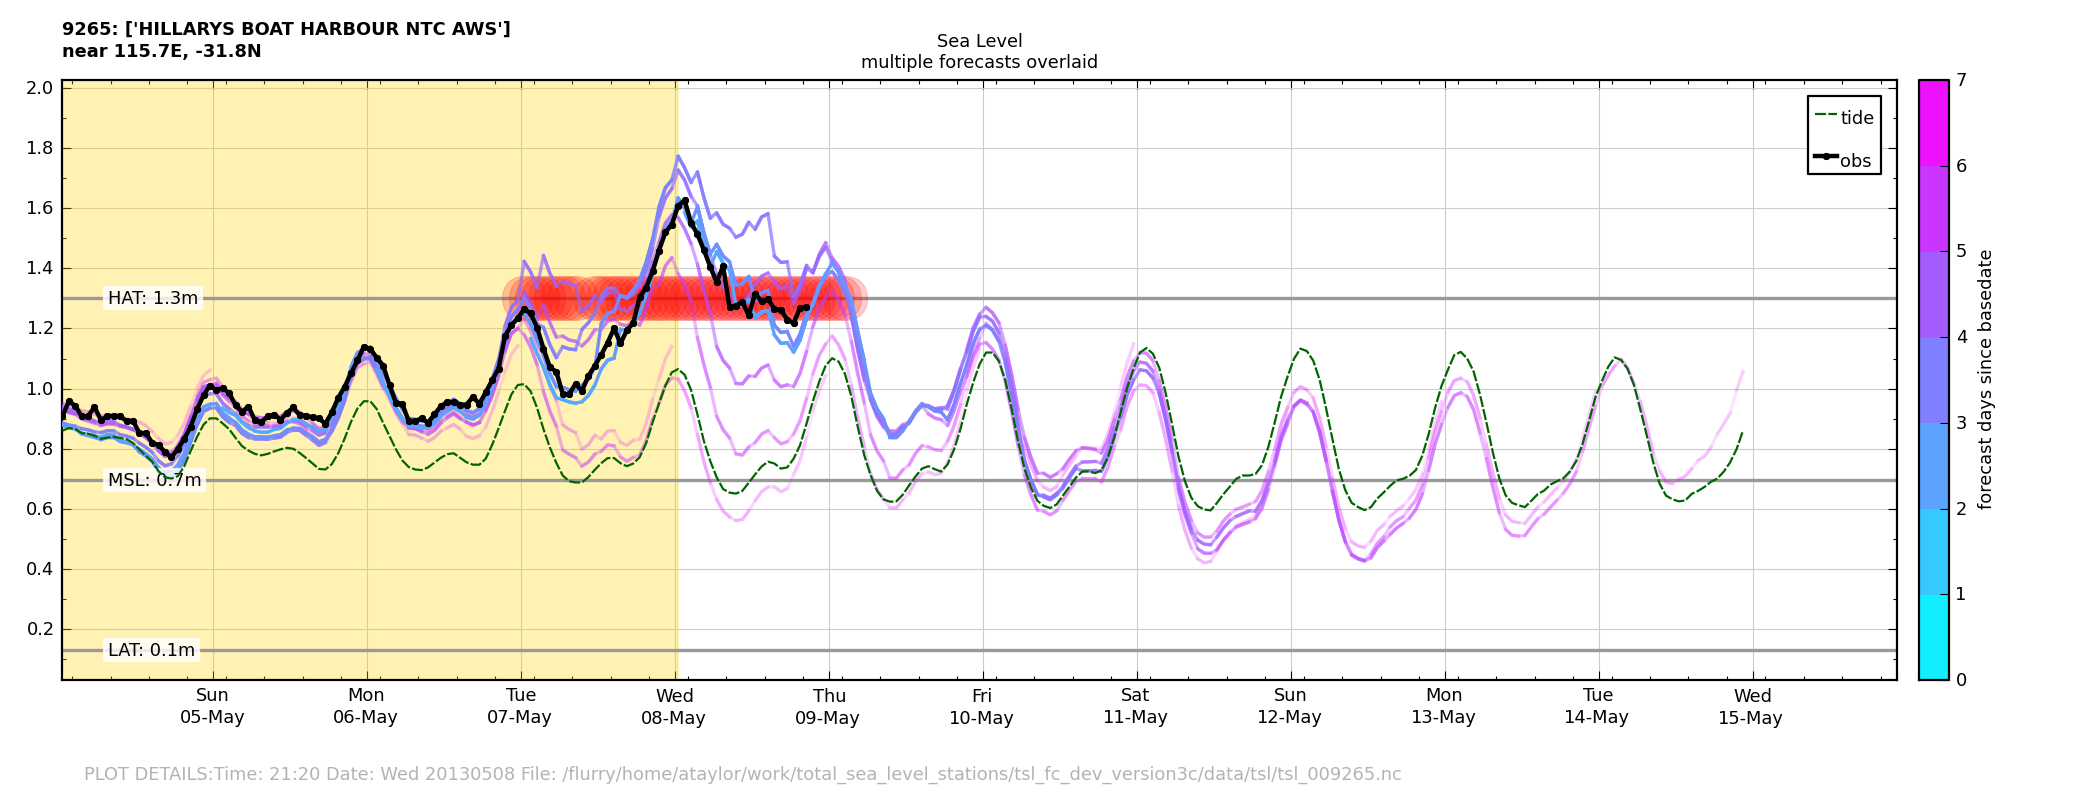
\includegraphics[width=150mm]{figures_3/aggregate_fc_plot_009265.png}
\caption{Aggregated sea level forecast example.   The harmonic tide component has been modified by the removal of certain constituents. Also of note is the spread of lagged-ensemble members related to forecast uncertainty.}
\label{fig:aggregated_fc}
\end{center}
\end{figure}


The motivation of this study is in effect the inverse of the previous problem [Section \ref{S:plan_nontidal_tidal}].  Put simply: {\bf how should harmonic analysis be approached in the context of \BL{}?}  \\
A premise of this work is that harmonic method will continue to provide a fundamental forecasting capability, but that details of implementation are worthy of re-examination in the context of the new prediction systems.\\

%Harmonic tide predictions are deterministic sea level forecasts based on observation statistics and an indirect connection to dynamical cause - as discussed in Section \ref{S:formalisms}.  



\subsubsection{Data sources}

This work will leverage the same data compiled for the study outlined in Section \ref{S:plan_nontidal_tidal}.  In summary:
\begin{itemize}
\item \BL{} operational outputs;
\item \OFAM{} spinup;
\item ABSLMP tide gauge and weather station historical data [Figure \ref{fig:ABSLMP}] ;
\item tidal constituents produced for the ANTT;
\end{itemize}

\subsubsection{Method outlook}

%This work will essentially approach tidal analysis from a conventional harmonic perspective.  In doing so, the approach will respond to the relatively recent publication of Foreman \citep{Foreman:2009bg} and the associated software.\\
Alternative approaches to preparing harmonic tide predictions for aggregation will be proposed and evaluated.\\


In the first instance, this will involve selective removal or attenuation of tidal constituents derived from the operational tidal analysis system of the \BOM{}.\\
Can aggregate forecast skill be improved by such a modification? \\
Note that in an attempt to put to one side the influence of barometric pressure, inverse barometer corrections will be applied based on observations rather than \NWP{} systems.\\ 



The problem will also be approached from a different angle. Can the estimation of nontidal sea level derived from \BL{} or \OFAM{} spinup be employed to improve the tidal analysis of observed sea level?\\
An estimate of non-tidal noise may be employed in a pre-processing step to adjust the observational record.  This has the prospect of reducing improper projection of turbulent signals onto the tidal basis. In practice this proposition raises several issues. \\
The statistical characterisation of an estimate of non-tidal `error' is significant; primarily with regard to the representative skill of estimate.  Another aspect involves the population statistics of the signal.  In the absence of any better estimate \citep{Foreman:2009bg} assumes a Gaussian error distribution - despite explicitly noting the lack of realism.  Statistics derived from the \BL{}  `lagged-ensemble' schedule will be explored with an eye to possible modifications to the formulation of the tidal projection formulation.




Ultimately, this work effort aims to recommend an approach to prepare or modify harmonic tides for aggregation.




